\renewcommand{\chaptername}{\scshape Partie}
\chapter{\normalfont \scshape Aspects organisationnels}
Afin d'assurer une bonne réalisation technique du projet, il a fallu rédiger un cahier des charges comprenant les livrables du projet, les risques et contraintes qui y sont liés, le matériel utilisé, le budget humain et financier, le diagramme de GANTT et enfin la répartition des tâches.
\section{Livrables \normalfont{\textit{(\emph{P}roduct \emph{B}reakdown \emph{S}tructure)}}}
Le livrable final comporte deux systèmes principaux : le montage d'imagerie Schlieren et le dispositif à onde de choc. Le PBS comprend donc le matériel nécessaire à chaque partie du projet, en plus du mode d'emploi. L'organigramme de la figure ~\ref{fig:PBS} représente le PBS prévu.
\begin{figure}[H]
	\begin{center}
	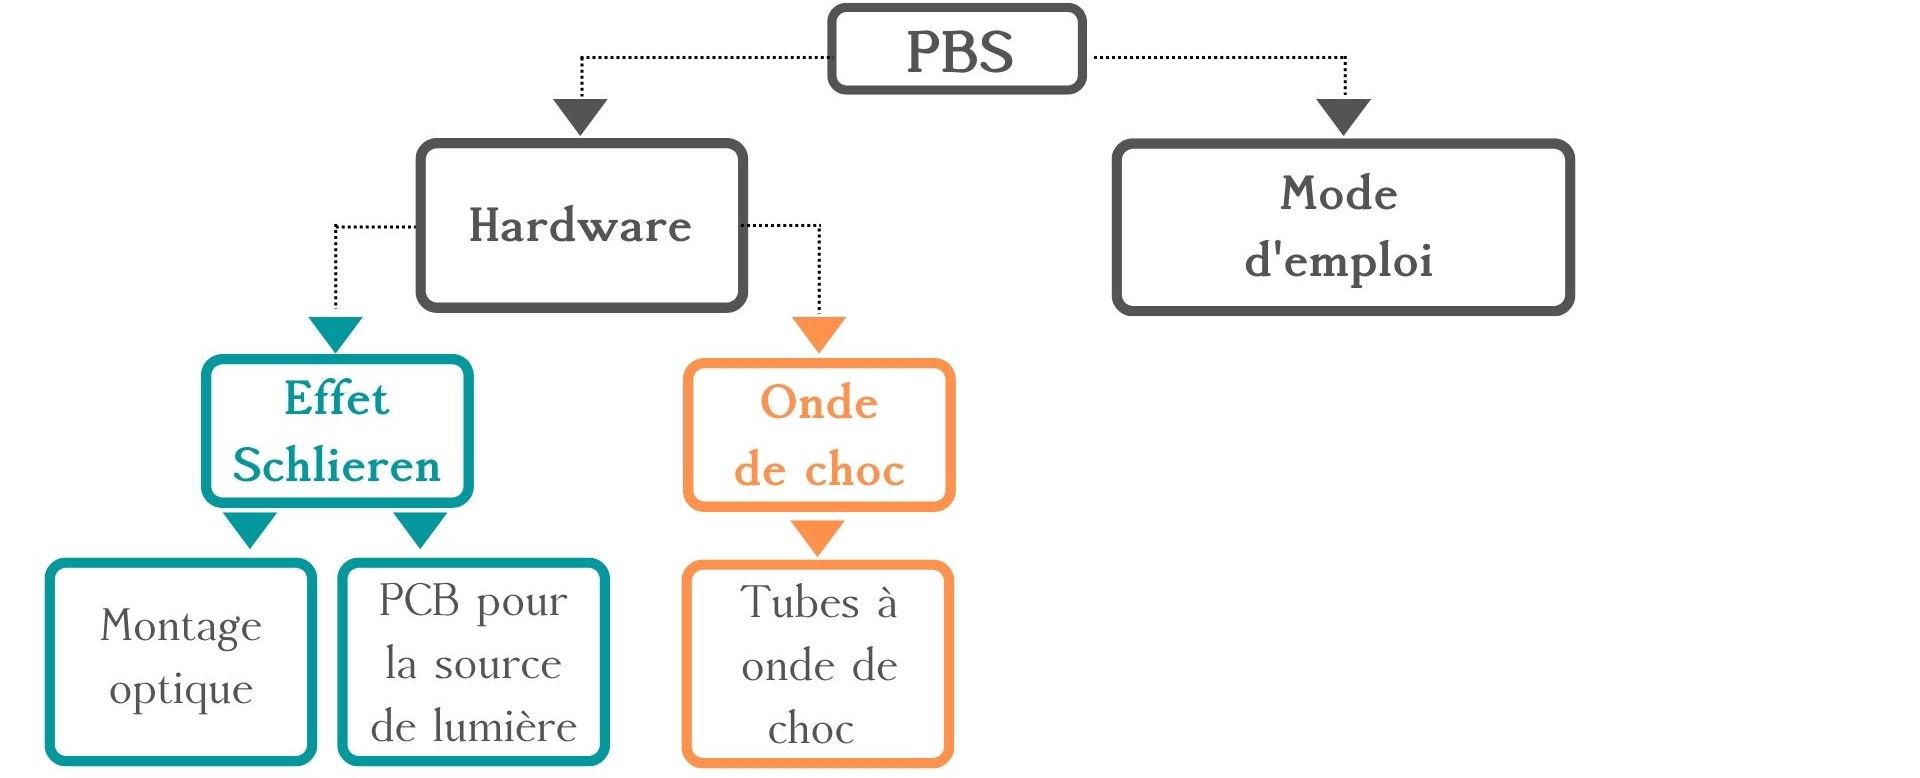
\includegraphics[scale = 0.2]{figures/PBS.jpg}
	\end{center}
	\caption{\small{\textit{Organigramme du PBS prévu}}}
	\label{fig:PBS}
\end{figure}
\section{Risques et contraintes}
Les tableaux ~\ref{tab:risques} et ~\ref{tab:contraintes} représentent respectivement les risques et les contraintes associés au projet ainsi que les mesures de prévention et les solutions d'optimisation :
\begin{table}[H]
	\centering
	\begin{tabular}{|l l l l|}
		\hline
		\small\textbf{Activité}&\vtop{\hbox{\strut \small\textbf{Équipement}}\hbox{\strut \small\textbf{utilisé}}}&\vtop{\hbox{\strut \small\textbf{Risques}}\hbox{\strut \small\textbf{associés}}}&\vtop{\hbox{\strut \small\textbf{Mesures de}}\hbox{\strut \small\textbf{prévention}}}\\
		\hline
		\vtop{\hbox{\strut \small{Réalisation du}}\hbox{\strut \small{tube à choc}}}&\small{Perceuse, scie}&\small{Blessure}&\vtop{\hbox{\small\strut Formation à l’utilisation du}\hbox{\small\strut matériel, gants de protection}}\\
		\hline
		\vtop{\hbox{\strut \small{Test de l'onde}}\hbox{\strut \small{de choc}}}&\vtop{\hbox{\strut \small{Air à pression }}\hbox{\strut \small{élevée (~5 bar)}}}&\vtop{\hbox{\strut \small{Explosion,}}\hbox{\strut \small{traumatisme sonore}}}&\vtop{\hbox{\small\strut Casque et/ou boules quies,}\hbox{\small\strut lunettes de protection}}\\
		\hline
		\vtop{\hbox{\strut \small{Réalisation des}}\hbox{\strut \small{différents dispositifs}}\hbox{\strut \small{du projet}}}&\vtop{\hbox{\strut \small{Ensemble du}}\hbox{\strut \small{matériel requis}}}&\vtop{\hbox{\strut \small{Matériel défectueux/}}\hbox{\strut \small{manquant}}}&\vtop{\hbox{\strut \small{Mieux labelliser les lentilles}}\hbox{\strut \small{et faire un inventaire}}\hbox{\strut \small{du matériel à Phelma}}}\\
		\hline
	\end{tabular}
	\caption{\small{\textit{Tableau récapitulatif des risques}}}
	\label{tab:risques}
\end{table}
\begin{table}[H]
	\centering
\begin{tabular}{|lll|}
	\hline
	\small\textbf{Types de contraintes}&\small\textbf{Description}&\small\textbf{Solutions}\\
	\hline
	\small{Contraintes budgétaires}&\vtop{\hbox{\strut \small{Miroir parabolique à}}\hbox{\strut \small{prix élevé et budget limité,}}\hbox{\strut \small{appareil photo à prix élevé}}}&\vtop{\hbox{\strut \small{Miroir de petit diamètre ou lentilles}}\hbox{\strut \small{convergentes (moins cher), prendre}}\hbox{\strut \small{un appareil photo d'un proche}}}\\
	\hline
	\small{Contraintes techniques}&\vtop{\hbox{\strut \small{Distance focale à déterminer}}\hbox{\strut \small{pour le miroir en salle de TP.}}}&\vtop{\hbox{\strut \small{Réalisation d'une source ponctuelle}}\hbox{\strut \small{afin de déterminer la distance focale.}}}\\
	&\small\vtop{\hbox{\strut \small{Nécessité d'une source}}\hbox{\strut \small{de lumière}}}&\vtop{\hbox{\strut \small{LED ou source de lumière}}\hbox{\strut \small{recouverte de papier aluminium}}}\\
	\hline
	\vtop{\hbox{\strut \small{Contraintes}}\hbox{\strut \small{organisationnelles}}}&\small{Tâches interdépendantes}&\vtop{\hbox{\strut \small{Répartition en groupes réalisant}}\hbox{\strut \small{les tâches simultanément}}} \\
	\hline
	\end{tabular}
	\caption{\small{\textit{Tableau récapitulatif des contraintes}}}
	\label{tab:contraintes}
\end{table}
\section{Matériel utilisé}
Une fois évalués, les risques et les contraintes permettent le choisir le matériel à utiliser de façon optimale. Pour réaliser le montage optique, le matériel suivant a été utilisé :
\begin{itemize}
	\item\textbf{Système optique :} Dans un premier temps, le choix a porté sur le miroir parabolique, étant donné qu'il est plus simple à utiliser en théorie que les lentilles convergentes. Une fois les tests sur le miroir effectués, une deuxième version du dispositif s'est basée sur les lentilles;
	\item\textbf{Sources lumineuses :} on a respectivement utilisé la lampe fournie en salle de TP, le flash d'un téléphone portable et une LED de forte intensité lumineuse;
	\item\textbf{Sources de chaleur :} Un briquet, une bougie et un sèche-cheveux;
	\item Un appareil photo.
\end{itemize}
Pour l'onde de choc, le matériel suivant a été utilisé :
